%From https://egu2018.eu/PICO_how-to_guide_to_PICO.pdf
%Abstracted and templated by Brian Ballsun-Stanton, Macquarie University.
%original template by https://github.com/snowtechblog/pico-latex-presentation by Anselm Köhler

\documentclass[unknownkeysallowed,usepdftitle=false,aspectratio=169, parskip=full]{beamer}
% unknownkeysallowed is needed for mac and the newer latex version -> is more picky than before...
\usetheme[headheight=1cm,footheight=2cm]{boxes}
%\usetheme{default}


\usepackage{default}
\usepackage{graphicx}
%example pictures created via: http://lorempixel.com/1200/800/cats/Figure2/. Credit to http://lorempixel.com/images.php

\usepackage{epsfig}
\usepackage{siunitx}
\usepackage{color}
\usepackage{ifthen}
\usepackage[rightcaption]{sidecap}
%usepackage{ragged2e}

\usepackage[T1]{fontenc}
\usepackage[utf8]{inputenc}
%https://tex.stackexchange.com/a/203804/5483

\usepackage[activate={true,nocompatibility},final,tracking=true,kerning=true,spacing=true,factor=1100,stretch=10,shrink=10]{microtype} % http://www.khirevich.com/latex/microtype/
\microtypecontext{spacing=nonfrench}

\usepackage{lipsum} % for dummy text only
\usepackage[UKenglish]{babel} %https://tex.stackexchange.com/a/27743 
\usepackage[pangram]{blindtext} % https://tex.stackexchange.com/a/48411

%\usepackage{parskip} % from https://tex.stackexchange.com/q/11622
%\setlength{\parskip}{12pt} 

%\setparsizes{\parindent}{12pt}{\parfillskip}

%\usepackage{etoolbox} % as per https://tex.stackexchange.com/a/24331
%\appto\chapterheadendvskip{\vspace{-1\parskip}}
%\setparsizes{\parindent}{50pt plus 20pt minus 30pt}{\parfillskip}

\setbeamertemplate{navigation symbols}{}%remove navigation symbols
\setbeamersize{text margin left=1cm,text margin right=1cm}

% some colors
\definecolor{grau}{gray}{.5}
\definecolor{slfcolor}{rgb}{0,0.6274,0.8353}
\definecolor{wslcolor}{rgb}{0,0.4,0.4}

% setup links
\hypersetup{%
	%linkbordercolor=green,%
	colorlinks=false,%
	pdfborderstyle={/S/U/W 0},%
	%pdfpagemode=FullScreen,%
	pdfstartpage=4%
	}

% setup some fonts
\setbeamerfont{title}{series=\bfseries, size=\small}
\setbeamerfont{author}{size*={5pt}{0pt}}
\setbeamerfont{institute}{size*={3pt}{0pt}}
\setbeamerfont{bodytext}{size=\scriptsize}
	
% Title setup	
\title{Corpus Word Frequency Analysis}
\author{Jan Jugueta (\texttt{jan.jugueta@hdr.mq.edu.au})}
\institute{Macquarie University, North Ryde, NSW}
% add title in headbox
\setbeamertemplate{headline}
{\leavevmode
\begin{beamercolorbox}[width=1\paperwidth]{head title}
  % LOGO
  \vspace{0.1cm}
  \begin{columns}[t, totalwidth=\textwidth]
  \begin{column}[c]{1.05cm}
     \includegraphics[width=1cm]{figure/logo1.png}
  \end{column}
  % TITLE
   \begin{column}[c]{10.6cm}
   \centering \usebeamerfont{title} \textcolor{slfcolor}{\inserttitle} \\
   \centering \usebeamerfont{author} \color[rgb]{0,0,0} \insertauthor \\
   \vspace{-0.05cm}
   \centering \usebeamerfont{institute} \insertinstitute
  \end{column}
  % PICTURE
  \begin{column}[c]{1.15cm}
    \hspace{0.005cm}
    \includegraphics[width=1cm]{figure/figure1.png}
  \end{column}
  \end{columns}
  {\color{slfcolor}\hrule height 1pt\vspace{0.1cm}}
\end{beamercolorbox}%
}

% setup the navigation in footbox
% first set some button colors
\newcommand{\buttonactive}{\setbeamercolor{button}{bg=wslcolor,fg=white}}
\newcommand{\buttonpassive}{\setbeamercolor{button}{bg=slfcolor,fg=black}}
% now set up that the one active one gets the new color.
\newcommand{\secvariable}{nothing}
% therefore we write before each section (well, everything which should be part of the navi bar)
% the variable \secvariable to any name which is in the next function ...
\newcommand{\mysection}[1]{\renewcommand{\secvariable}{#1}
}
% ... compaired to strings in the following navibar definition ...
\newcommand{\tocbuttoncolor}[1]{%
 \ifthenelse{\equal{\secvariable}{#1}}{%
    \buttonactive}{%
    \buttonpassive}
 }
% ... here we start to set up the navibar. each entry is calling first the function \tocbuttoncolor with the argument which should be tested for beeing active. if active, then change color. afterwards the button is draw. so to change that, you need to change the argument in \toc..color, the first in \hyperlink and before each frames definition... A bit messed up, but works...
\newlength{\buttonspacingfootline}
\setlength{\buttonspacingfootline}{-0.2cm}
\setbeamertemplate{footline}
{\leavevmode
\begin{beamercolorbox}[width=1\paperwidth]{head title}
  {\color{slfcolor}\hrule height 1pt}
  \vspace{0.05cm}
  % set up the buttons in an mbox
  \centering \mbox{
    \tocbuttoncolor{abstract}
    \hyperlink{abstract}{\beamerbutton{2 Minute Madness}}
    \tocbuttoncolor{radar}
    \hspace{\buttonspacingfootline}
      \hyperlink{radar}{\beamerbutton{Section 1}}

    \tocbuttoncolor{line}
    \hspace{\buttonspacingfootline}
      \hyperlink{line}{\beamerbutton{Section 2}}
    \tocbuttoncolor{major}
    \hspace{\buttonspacingfootline}
      \hyperlink{major}{\beamerbutton{Section 3}}
    \tocbuttoncolor{slab}
    \hspace{\buttonspacingfootline}
      \hyperlink{slab}{\beamerbutton{Section 4}}
    \tocbuttoncolor{minor}
    \hspace{\buttonspacingfootline}
      \hyperlink{minor}{\beamerbutton{Section 5}}
    \tocbuttoncolor{conclusion}
    \hspace{\buttonspacingfootline}
      \hyperlink{conclusion}{\beamerbutton{Conclusion}}
    % this last one should normaly not be used... it will open the preferences to change the 
    % behaviour of the acrobat reader in fullscreen -> usefull in pico...
    \setbeamercolor{button}{bg=white,fg=black}
    % for presentation
    %\hspace{-0.1cm}\Acrobatmenu{FullScreenPrefs}{\beamerbutton{\#}}
    % for upload
    
     
\Acrobatmenu{FullScreenPrefs}{\vspace{0.3cm}\hspace{0.24cm}\mbox{%
      
\includegraphics[height=0.04\textheight,keepaspectratio]{%
	  figure/CreativeCommons_Attribution_License.eps}%
	  }}
   }
    \vspace{0.05cm}
\end{beamercolorbox}%
}


\begin{document}


%%%%%%%%%%%%%%%%%%%%%%%%%%%%%%%%%%%%%%%%%%%%%%%%%%%%%%%%%%%%%%%%%%%%%%%%%%
\mysection{abstract}
%%%%%%%%%%%%%%%%%%%%%%%%%%%%%%%%%%%%%%%%%%%%%%%%%%%%%%%%%%%%%%%%%%%%%%%%%%
\begin{frame}\label{\secvariable}
\begin{center}
\begin{figure}[h]
\centering
\includegraphics[width=0.8\textwidth,height=0.8\textheight,keepaspectratio]{figure/nd.png}
\caption{Five front pages from \textit{Neues Deutschland}. Adapted from Neues Deutschland, by Jan Jugueta, 2019, retrieved from http://nd-archiv.de/. Copyright 1974 by Neues Deutschland.}
\end{figure}
\end{center}
\end{frame}

\begin{frame}\label{\secvariable}
  \begin{columns}[t]
  %https://tex.stackexchange.com/a/7452/5483
  \begin{column}[c]{0.45\textwidth}
%http://lorempixel.com/1200/800/cats/Figure2/     
%http://lorempixel.com/1200/800/cats/Figure3/
\includegraphics[width=1\textwidth,height=0.5\textheight,keepaspectratio]{%
figure/logo1.png}\\
\vspace{12pt}
\includegraphics[width=1\textwidth,height=0.5\textheight,keepaspectratio]{%
figure/figure1.png}
    \end{column}
    \begin{column}[c]{0.45\textwidth}
    \parbox{\linewidth}{

      Integer dictum condimentum elit ac placerat. Duis vitae ex nec mauris iaculis maximus. Aliquam est velit, imperdiet placerat velit elementum, fringilla fringilla tortor. Nunc tempus vulputate leo, ac commodo dolor mattis ullamcorper. Donec elementum dapibus justo ut vestibulum. 
      
      \vspace{12pt}
      
      Phasellus aliquam porta justo, et accumsan libero tristique quis. Aenean vel risus accumsan, feugiat lorem vel, placerat.
      }
    \end{column}
    
  \end{columns}

  
\end{frame}

%%%%%%%%%%%%%%%%%%%%%%%%%%%%%%%%%%%%%%%%%%%%%%%%%%%%%%%%%%%%%%%%%%%%%%%%%%
\mysection{radar}
%%%%%%%%%%%%%%%%%%%%%%%%%%%%%%%%%%%%%%%%%%%%%%%%%%%%%%%%%%%%%%%%%%%%%%%%%%
\begin{frame}\label{\secvariable}
  \begin{columns}[t]
  %https://tex.stackexchange.com/a/7452/5483
    \begin{column}[c]{0.45\textwidth}
    \parbox{\linewidth}{

      Donec dignissim vel ligula a sollicitudin. Donec rutrum faucibus dictum. Quisque in pellentesque massa. Aliquam mi lectus, facilisis sit amet dignissim vitae, porta vitae elit. Nulla nulla nunc, consectetur a blandit nec, aliquam ultrices dolor. Duis pellentesque urna ut sem lobortis maximus.
      
      \vspace{12pt}
      
	  Some extra words demonstrating a paragraph. The quick brown fox jumps over the lazy dog.
      }
    \end{column}
    \begin{column}[c]{0.45\textwidth}
%http://lorempixel.com/1200/800/cats/Figure2/     
%http://lorempixel.com/1200/800/cats/Figure3/
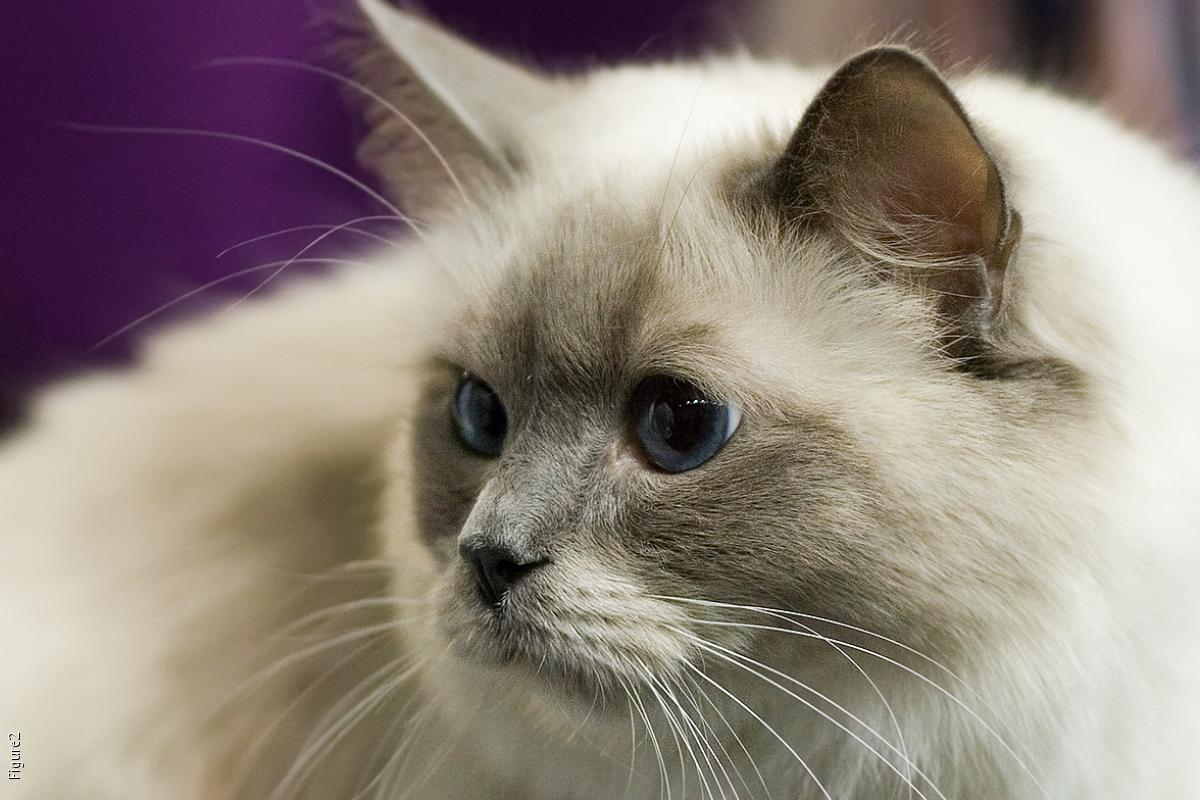
\includegraphics[width=1\textwidth,height=0.5\textheight,keepaspectratio]{%
figure/figure2.png}\\
\vspace{12pt}
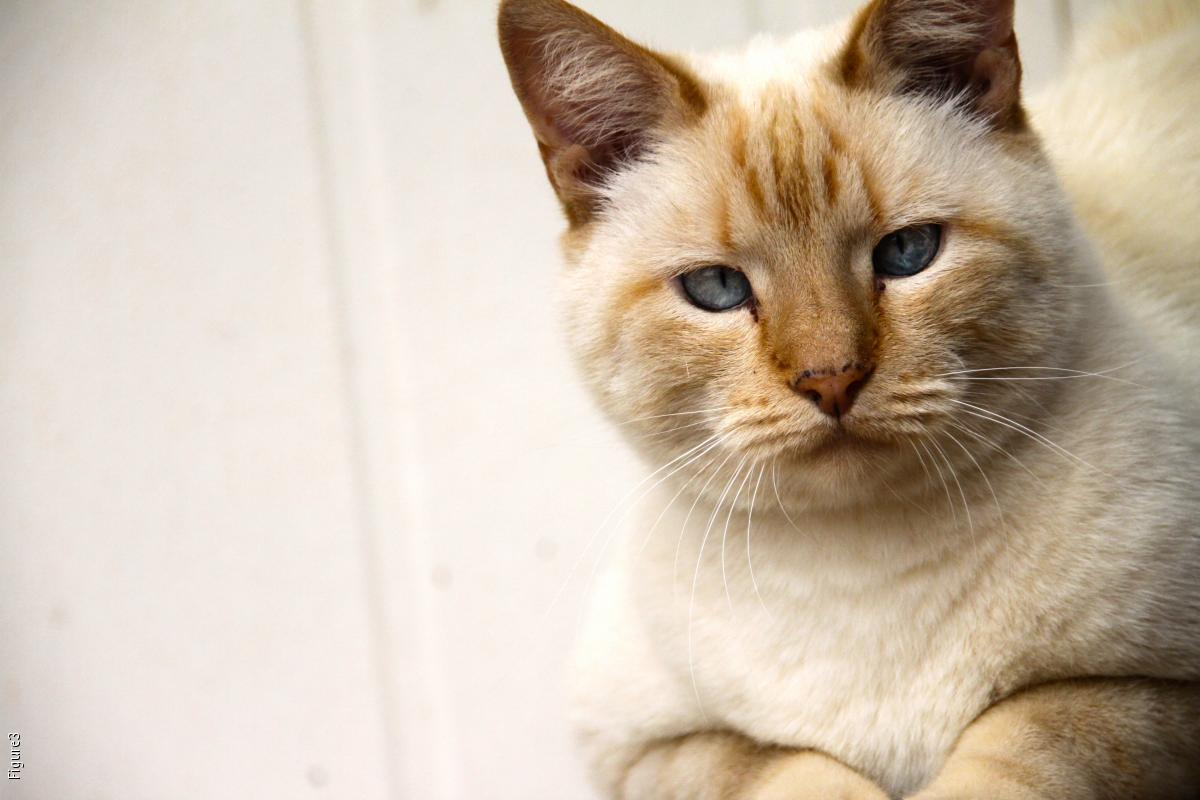
\includegraphics[width=1\textwidth,height=0.5\textheight,keepaspectratio]{%
figure/figure3.png}
    \end{column}
  \end{columns}

  
\end{frame}

%%%%%%%%%%%%%%%%%%%%%%%%%%%%%%%%%%%%%%%%%%%%%%%%%%%%%%%%%%%%%%%%%%%%%%%%%%
\mysection{line}
%%%%%%%%%%%%%%%%%%%%%%%%%%%%%%%%%%%%%%%%%%%%%%%%%%%%%%%%%%%%%%%%%%%%%%%%%%
\begin{frame}\label{\secvariable}
\begin{center}
  \vspace{-0.5cm}
  %http://lorempixel.com/1200/800/cats/Figure4/
 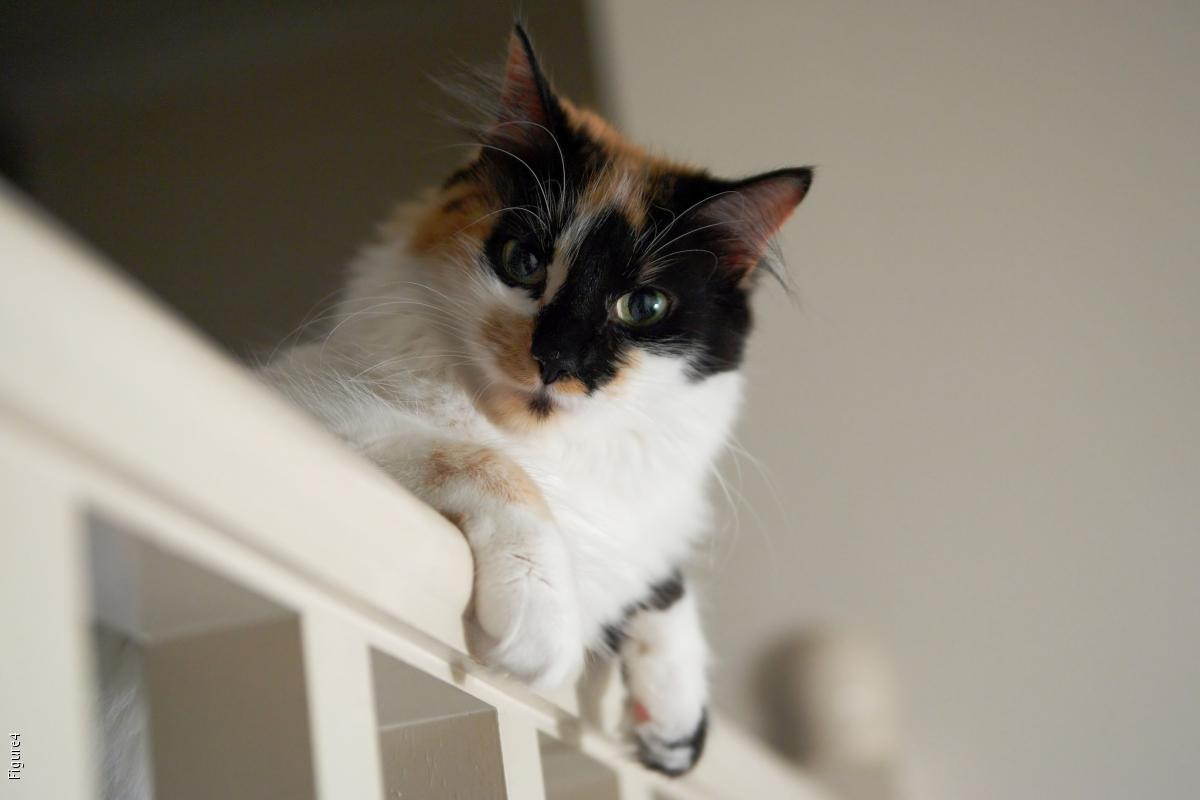
\includegraphics[width=1\textwidth,height=0.75\textheight,keepaspectratio]{%
  figure/figure4.png}
\end{center}
  \vspace{-0.5cm}
  \begin{enumerate}[(a)]
  
  
  \item Morbi vehicula ornare augue vitae porttitor.
  \item Donec porttitor, nibh id pretium euismod,
  \end{enumerate}

  $\quad \Rightarrow$ Aliquam et turpis eget lacus finibus congue.
  
\end{frame}

%%%%%%%%%%%%%%%%%%%%%%%%%%%%%%%%%%%%%%%%%%%%%%%%%%%%%%%%%%%%%%%%%%%%%%%%%%
\mysection{major}
%%%%%%%%%%%%%%%%%%%%%%%%%%%%%%%%%%%%%%%%%%%%%%%%%%%%%%%%%%%%%%%%%%%%%%%%%%
\begin{frame}\label{\secvariable} %%Eine Folie
\begin{center}
%http://lorempixel.com/1200/800/cats/Figure5/
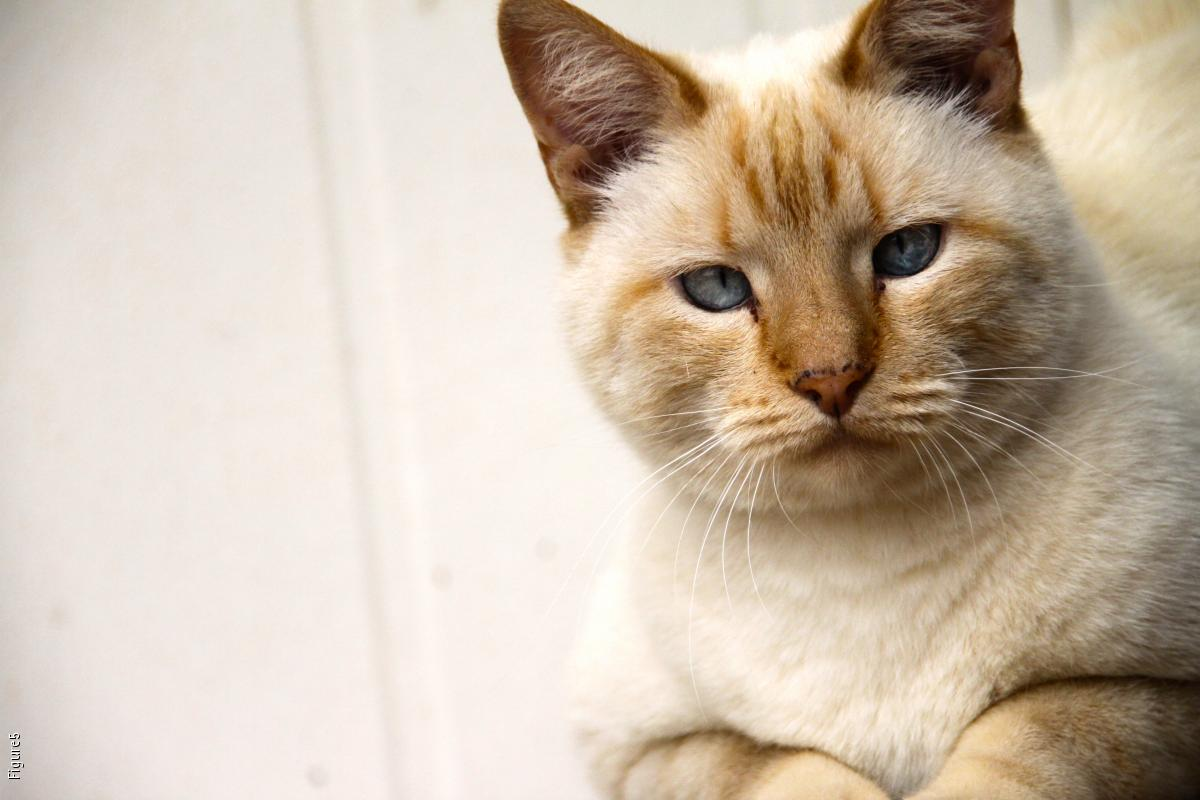
\includegraphics[width=1\textwidth,height=0.8\textheight,keepaspectratio]{%
figure/figure5.png}
\end{center}

    \parbox{\linewidth}{

Vivamus efficitur ac odio ac scelerisque. Sed tristique vel sapien euismod elementum. Donec eu mollis mi, et auctor est.
}
\end{frame}

%%%%%%%%%%%%%%%%%%%%%%%%%%%%%%%%%%%%%%%%%%%%%%%%%%%%%%%%%%%%%%%%%%%%%%%%%%
\mysection{slab}
%%%%%%%%%%%%%%%%%%%%%%%%%%%%%%%%%%%%%%%%%%%%%%%%%%%%%%%%%%%%%%%%%%%%%%%%%%
\begin{frame}\label{\secvariable}
%http://lorempixel.com/1200/800/cats/Figure6/
\begin{center}
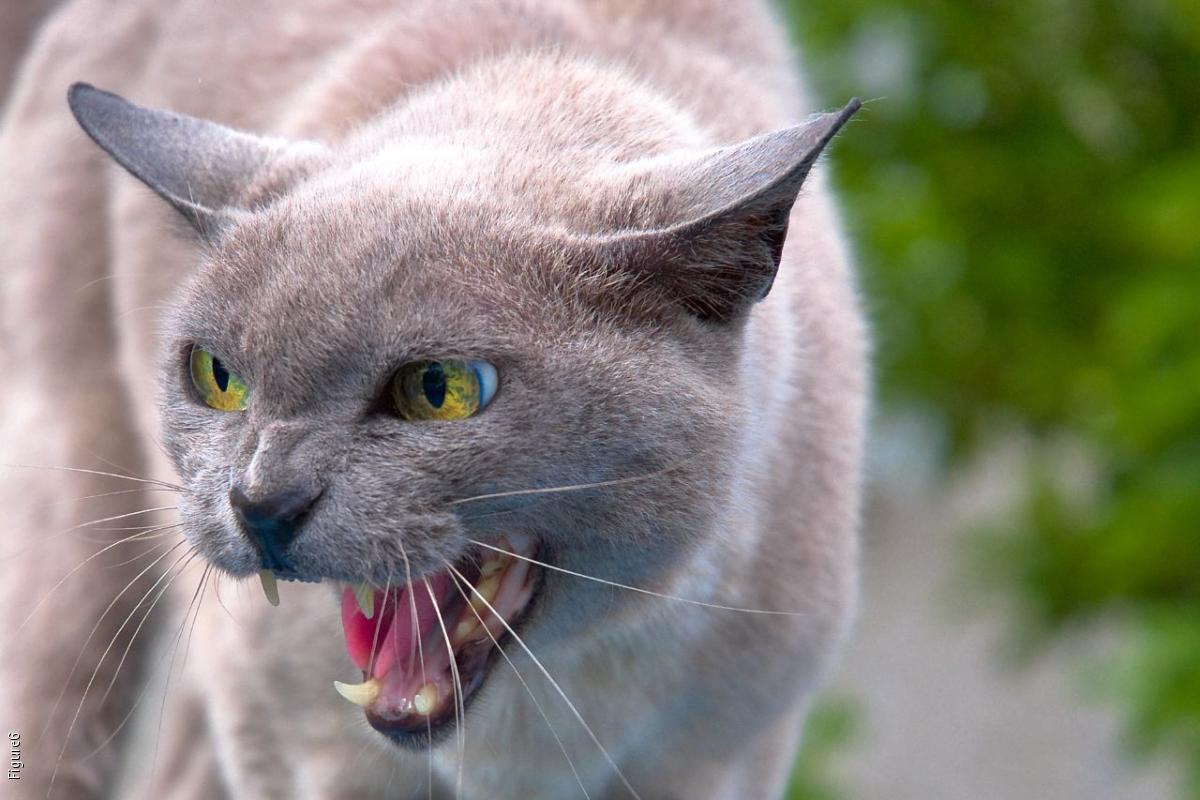
\includegraphics[width=1\textwidth,height=0.75\textheight,keepaspectratio]{%
figure/figure6.png}
\end{center}
    \parbox{\linewidth}{

Etiam cursus nibh nec ex tincidunt pharetra quis vel nibh. Sed condimentum lobortis mollis. Donec vitae odio nec lacus iaculis condimentum. Proin dictum consequat quam nec. \hyperlink{slabtable}{\beamerbutton{more \dots}}
}

\end{frame}



\begin{frame}\label{slabtable}
\begin{columns}
\begin{column}[t]{1.1\textwidth}
\hyperlink{slab}{\beamerbutton{\dots back to figure}}\\
Morbi mauris turpis, ornare eu elit quis, pulvinar bibendum sapien. Nulla vel justo id dui aliquam blandit. Etiam pellentesque ac nisl ut suscipit. 


%Table from original template.

\vspace{0.3cm}
\end{column}
\end{columns}
\usebeamerfont{bodytext}
 \begin{tabular}{c|rr@{}c@{}rrrrr}
 \setlength{\tabcolsep}{6mm}
   & Time & \multicolumn{3}{r}{Volume} & Range & Length & Area & Depth \\
   & [\si{\second}] & \multicolumn{3}{r}{[\si{\cubic\metre}]} & [\si{\metre}] &
[\si{\metre}] & [\si{\square\metre}] & [\si{\metre}]\\\hline

   \textbf{Avalanche~\#0019} & & $V_t$ &=& 29500 & & & 40411 & 0.73 \\
   initial release &3.4& $V_0$ &=& 2188 & 2506 &  62 &  1400 & 1.56 \\
   slab \#1 & 17.2    &  $V_1$ &=&  521 & 2356 &  39 &   701 & 0.74 \\
   slab \#2 & 23.4    &  $V_2$ &=& 3503 & 2284 &  83 &  2753 & 1.28 \\
   slab \#3 & 20--25$^*$ &  $V_3$ &=& 3345 & 2150 &  99 &  1880 & 1.78 \\
   slab \#4 & 38.7    &  $V_4$ &=& 4276 & 1945 & 153 &  3657 & 1.17 \\
   \\
   \textbf{Avalanche~\#0017} & &  $V_t$ &=& 78500 & & & 82632 & 0.95\\
   initial release&5.2&  $V_0$ &=& 15233 & 2402 & 191 & 12974 & 1.17\\
   slab \#5 & 12.2    &  $V_5$ &=&  7620 & 2219 & 202 &  6043 & 1.26 \\
   slab \#6 & 14.1    &  $V_6$ &=&  5868 & 2215 & 166 &  5851 & 1.01 \\
   slab \#7 & 25.6    &  $V_7$ &=&  6307 & 1982 &  95 &  3320 & 1.90 \\
   slab \#8 & 15--25$^*$ &  $V_8$ &=& 10663 & 1947 & 253 &  5037 & 2.12
 \end{tabular}
 
\vspace{0.2cm}
 \textbf{Table:} Release time, Volume, Location and size parameters of all
identified slabs.

\end{frame}




%%%%%%%%%%%%%%%%%%%%%%%%%%%%%%%%%%%%%%%%%%%%%%%%%%%%%%%%%%%%%%%%%%%%%%%%%%
\mysection{minor}
%%%%%%%%%%%%%%%%%%%%%%%%%%%%%%%%%%%%%%%%%%%%%%%%%%%%%%%%%%%%%%%%%%%%%%%%%%
\begin{frame}\label{\secvariable} %%Eine Folie
\begin{center}
%http://lorempixel.com/1200/800/cats/Figure7/
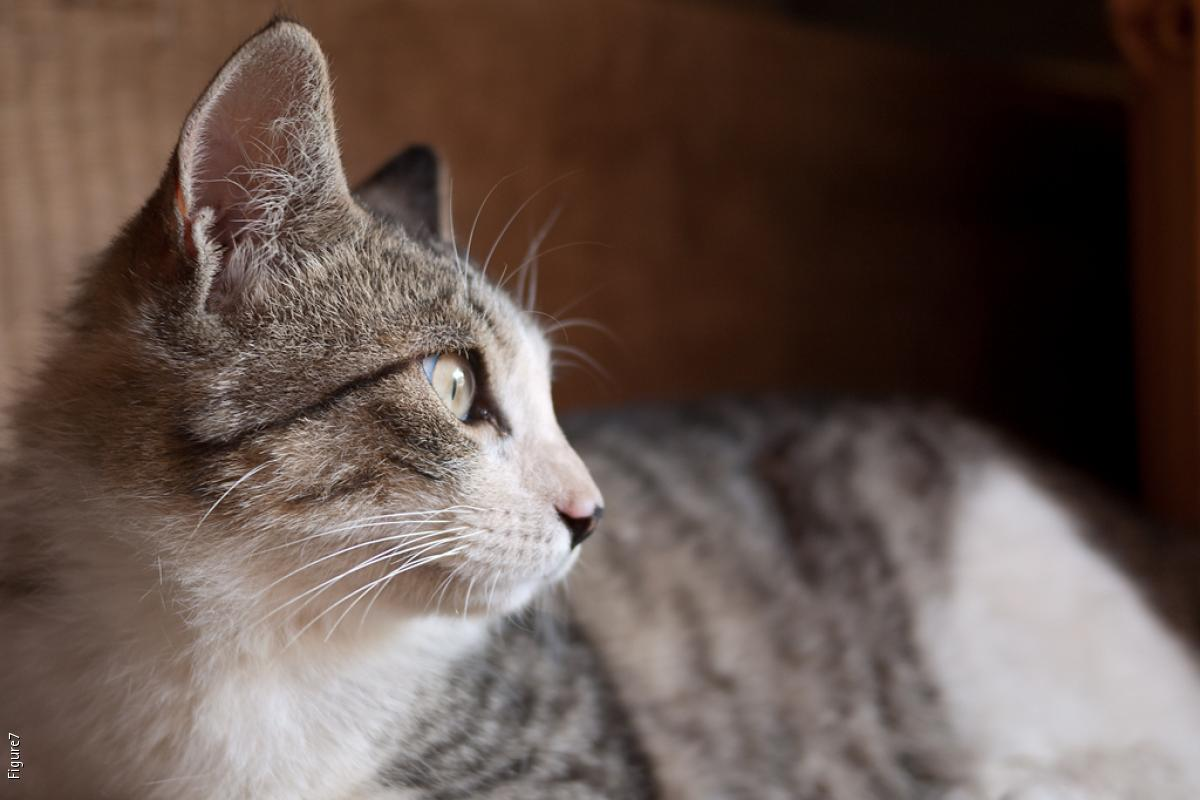
\includegraphics[width=1\textwidth,height=0.7\textheight,keepaspectratio]{%
figure/figure7.png}
\end{center}
\vspace{-0.2cm}

Duis condimentum est id nulla dapibus semper. Maecenas in tellus eget purus egestas fringilla in vitae nisl. Nulla vulputate tempor purus ut finibus. Nunc gravida placerat tortor vel efficitur. Sed tincidunt enim sed nisl hendrerit vestibulum. 

\end{frame}

%%%%%%%%%%%%%%%%%%%%%%%%%%%%%%%%%%%%%%%%%%%%%%%%%%%%%%%%%%%%%%%%%%%%%%%%%%

%%%%%%%%%%%%%%%%%%%%%%%%%%%%%%%%%%%%%%%%%%%%%%%%%%%%%%%%%%%%%%%%%%%%%%%%%%
\begin{frame}\label{\secvariable}

%
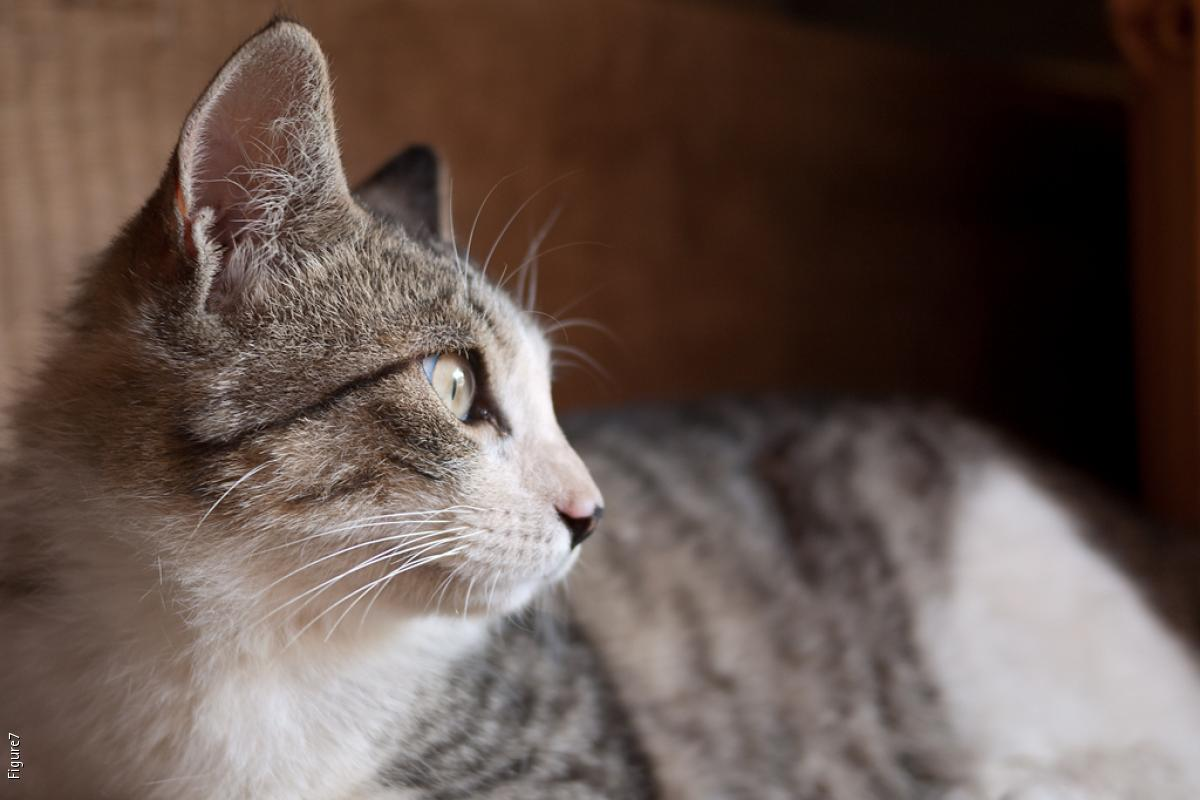
\includegraphics[width=0.45\textwidth,height=1\textheight,keepaspectratio]{%
figure/figure7.png}\hspace{.05\textwidth}
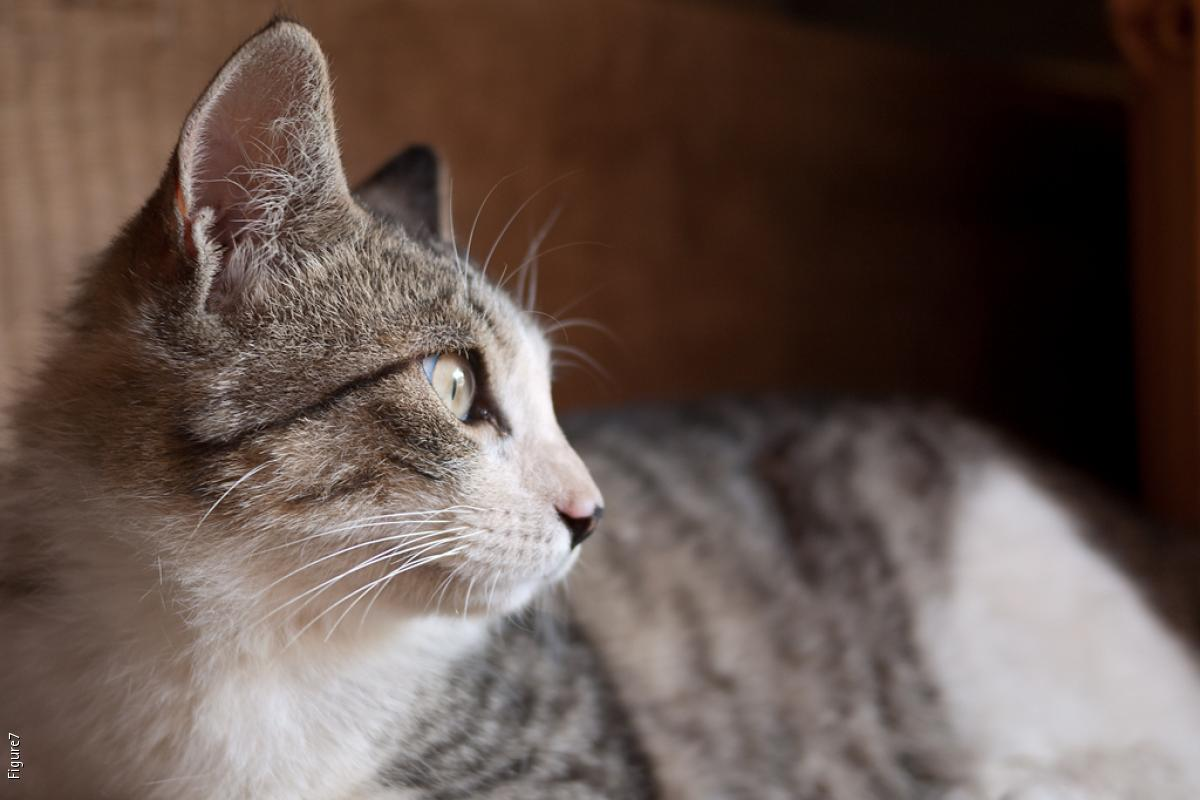
\includegraphics[width=0.45\textwidth,height=1\textheight,keepaspectratio]{%
figure/figure7.png}

Maecenas nec accumsan nunc. Aenean pretium nulla augue, sit amet volutpat leo consectetur tincidunt. Donec scelerisque erat a semper lacinia. Pellentesque aliquet libero neque, ac consequat metus feugiat eget. Etiam aliquam maximus libero, quis hendrerit ex mattis vitae. Duis sed metus ultrices, hendrerit sapien vitae, fringilla nunc. 

\end{frame}

%%%%%%%%%%%%%%%%%%%%%%%%%%%%%%%%%%%%%%%%%%%%%%%%%%%%%%%%%%%%%%%%%%%%%%%%%%
\mysection{conclusion}
%%%%%%%%%%%%%%%%%%%%%%%%%%%%%%%%%%%%%%%%%%%%%%%%%%%%%%%%%%%%%%%%%%%%%%%%%%
\begin{frame}\label{\secvariable}
  
  \begin{itemize}
   \item Curabitur viverra massa vel elit tincidunt lacinia. Pellentesque id est lobortis, interdum felis nec, faucibus augue. Suspendisse varius sit amet dui ac dignissim. Quisque mattis, odio a congue lobortis, eros turpis placerat enim, ac tempor lorem nisl ut velit. Mauris vel nulla a quam viverra faucibus. 
  \item Quisque sed orci eu libero mattis lobortis. Curabitur aliquam lorem neque, ac auctor justo sagittis sed. Nunc augue nisl, mattis sed turpis at, elementum lobortis augue. Vestibulum porta felis bibendum mattis iaculis. Nulla dignissim varius rutrum.
  \item Vivamus eget semper nunc. Donec sodales ornare porttitor. Curabitur commodo viverra arcu. Aliquam consequat felis non dolor consequat ultricies. Mauris non finibus nisl. Sed tincidunt felis at porttitor posuere.

  \end{itemize}

  \usebeamerfont{bodytext}
  K\"ohler, A., J. N. McElwaine, B. Sovilla, M. Ash, P. Brennan (in Review),
Surge dynamics of the 3 February 2015 avalanches in Valle\'e de la Sionne,
\textit{J. Geophys. Res.} 
  
\end{frame}



\end{document}
